\documentclass[11pt]{article}
\usepackage{latexsym}
\usepackage{amsmath}
\usepackage{amssymb}
\usepackage{amsthm}

\usepackage{listings}[language=Python]
\usepackage{pifont}% http://ctan.org/pkg/pifont
\newcommand{\xmark}{\text{\ding{55}}}
\newcommand{\cmark}{\text{\ding{51}}}
\newcommand{\tri}{\text{\ding{115}}}

\usepackage{epsfig}
\usepackage[tight]{subfigure}

\usepackage{bm}
\usepackage{graphicx}
\usepackage{caption}
\usepackage{subcaption}
\usepackage{float}


\usepackage{amsmath}

\DeclareMathOperator*{\minimize}{min}
\DeclareMathOperator*{\maximize}{max}

\usepackage{algorithm}
 %on linux you may need to run sudo apt-get install texlive-full to install algorithm.sys
\usepackage{algorithmic}

\usepackage{verbatim}

\newcommand{\handout}[5]{
  \noindent
  \begin{center}
  \framebox{
    \vbox{
      \hbox to 5.78in { {#1} \hfill #2 }
      \vspace{4mm}
      \hbox to 5.78in { {\Large \hfill #5  \hfill} }
      \vspace{2mm}
      \hbox to 5.78in { {\em #3 \hfill #4} }
    }
  }
  \end{center}
  \vspace*{4mm}
}

\newcommand{\lecture}[5]{\handout{#1}{#2}{#3}{#4}{#5}}
\newcommand{\collision}[0]{\mathrm{collision}}
\newcommand{\nocollision}[0]{\overline{\collision}}

\newcommand*{\QED}{\hfill\ensuremath{\square}}

\newtheorem{theorem}{Theorem}
\newtheorem{corollary}[theorem]{Corollary}
\newtheorem{lemma}[theorem]{Lemma}
\newtheorem{observation}[theorem]{Observation}
\newtheorem{proposition}[theorem]{Proposition}
\newtheorem{definition}[theorem]{Definition}
\newtheorem{claim}[theorem]{Claim}
\newtheorem{fact}[theorem]{Fact}
\newtheorem{assumption}[theorem]{Assumption}
\newtheorem{note}[theorem]{Note}

% 1-inch margins, from fullpage.sty by H.Partl, Version 2, Dec. 15, 1988.
\topmargin 0pt
\advance \topmargin by -\headheight
\advance \topmargin by -\headsep
\textheight 8.9in
\oddsidemargin 0pt
\evensidemargin \oddsidemargin
\marginparwidth 0.5in
\textwidth 6.5in

\parindent 0in
\parskip 1.5ex
%\renewcommand{\baselinestretch}{1.25}

\begin{document}

\lecture{Statistical Techniques in Robotics (16-831, S22)}{Lecture \#14
  (Monday, March 14)}{Lecturer: Kris Kitani}{Scribes: Xuanbai Chen, Jia Shi (Group C)}{Sequence Feedback Learning Problems: MDP}

\section{Review}
In the last lecture, we talked about Thompson Sampling, EXP3 and EXP4 algorithms.
\subsection{Thompsons Sampling: Beta-Bernoulli Bandit}
The algorithm is shown below:
\begin{algorithm}[H]
\caption{Bern-Beta Thompsons Sampling}
\label{algo:thompson}
\begin{algorithmic}[1]

\FOR{$t=1,\;\cdots,\;T$}
\STATE $\theta_k \sim p(\thata; \alpha_k, \beta_k) \quad \forall k$ \quad \text{sample from posterior} 
\STATE $a_{\hat{k}}^{(t)} = argmax_k \mathbb{E}_{p(r \mid a_k, \theta_k)} \left[r \mid a_k, \theta_k \right]$\quad \text{}
\STATE $\textsc{RECEIVE}(r^{(t)})$ \quad \text{get sampled reward}
\STATE $\alpha_{\hat{k}} = \alpha_{\hat{k}} + r^{(t)}$ \quad \text{update posterior}
\STATE $\beta_{\hat{k}} = \beta_{\hat{k}} + 1 - r^{(t)}$ \quad \text{update posterior}
\ENDFOR

\end{algorithmic}
\end{algorithm}
It is a no-regret algorithm with the regret bound of:
$$BR \le O(\sqrt{TK \log T})$$

\subsection{EXP3 - Exponential-Weight Update algorithm for Exploration and Exploitation}
EXP3 is designed for sampling action in context-free adversarial environment. The algorithm is listed as below.
\begin{algorithm}[H]
\caption{EXP3(\gamma \in [0, 1])}
\label{algo:exp3}
\begin{algorithmic}[1]
\STATE $\textbf{w}^{(1)}$ \leftarrow $\{w_k^{(1)} = 1 \}_{k=1}^K$ \quad \text{weights over actions}
\FOR{$t=1,\;\cdots,\;T$}
\STATE $\textbf{p}^{(t)} = \frac{\textbf{w}^{(t)}}{\sum_k w_k^{(t)}}$ \quad \text{probability over actions}
\STATE k $\sim  \textsc{MULTINOMIAL}(\textbf{p}^{(t)})$ \quad \text{take and draw action}
\STATE $a^{(t)} = a_k$ 
\STATE $\textsc{RECEIVE}(r^{(t)}\in[0, 1])$ \quad \text{get reward}
\STATE $w_k^{(t+1)} = w_k^{(t)}e^{\gamma \frac{r^{(t)}}{p_k^{(t)}}}$ \quad \text{update weight for one arm}
\ENDFOR
\end{algorithmic}
\end{algorithm}

The EXP3 is a no regret algorithm by setting
$$\gamma = \sqrt{\frac{\log K}{TK}},$$
the regret bound is
$$R \le O(\sqrt{TK \log K}).$$

\subsection{EXP4 - Exponential-Weight Update algorithm for Exploration and Exploitation with  Experts}
EXP4 algorithm is designed for contextual Multi-Arm Bandit problem, whose algorithm is listed below:
\begin{algorithm}[H]
\caption{EXP4(\gamma \in [0, 1], T)}
\label{algo:exp4}
\begin{algorithmic}[1]
\STATE $\textbf{w}^{(1)} \leftarrow \textbf{1} \in \mathbb{R}^N$ \quad \text{weights over experts}
\FOR{$t=1,\;\cdots,\;T$}
\STATE $\textsc{RECEIVE}( X^{(t)}\in \mathbb{R}^{N \times K})$ \quad \text{advice from N experts}
\STATE $\textbf{q}^{(t)} = \frac{\textbf{w}^{(t)}}{\|\textbf{w}^{(t)}\|}$ \dot $ \textbf{X}^{(t)} \in \Delta^K$ \quad \text{probability over actions}
\STATE k^{(t)} $\sim  \textsc{MULTINOMIAL}(\textbf{q}^{(t)})$ \quad \text{draw action}
\STATE $\textsc{RECEIVE}(r^{(t)})$ \quad \text{get reward}
\STATE $\hat{\textbf{r}}^{(t)} = \frac{r^{(t)}}{q_k^{(t)}}\mathbb{I}[k = k^{(t)}] \in \mathbb{I}^K$ \quad \text{reward over all arms}
\STATE $\textbf{g}^{(t)} = \textbf{X}^{(t)} \dot \hat{\textbf{r}}^{(t)} \in \mathbb{R}^N$ \quad \text{per expert reward}
\STATE $w_k^{(t+1)} = w_k^{(t)}e^{\gamma g_n^{(t)}} \quad \forall n$ 
\ENDFOR
\end{algorithmic}
\end{algorithm}
The regret bound of EXP4 is 
$$R_{EXP4} \le \sqrt{KT \log N}.$$

\section{Summary}
\begin{figure}[H]
\centering
    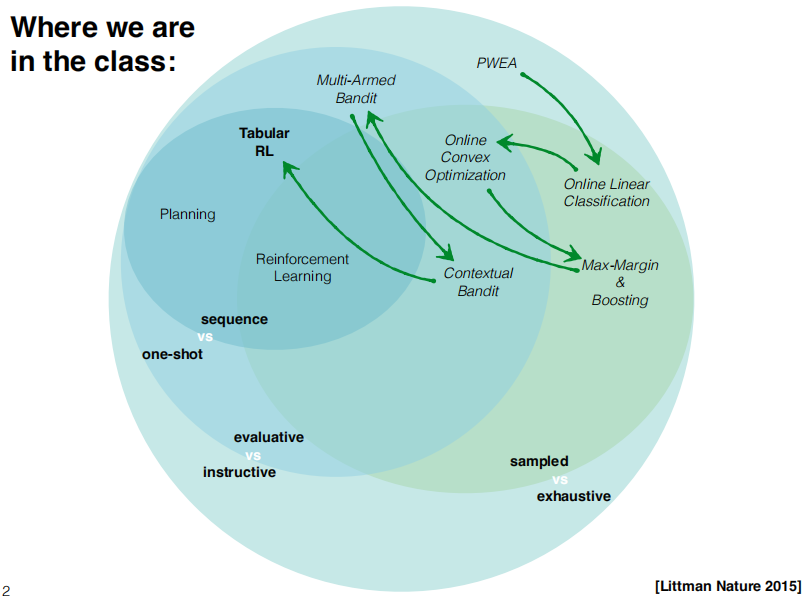
\includegraphics[width=0.7\textwidth]{1.png}
    \caption{The knowledge that we have covered up to now.}
	\label{fig:3.2-original}
\end{figure}

\subsection{Comparison SL vs RL}
Up to now, we have studied several online learning algorithms to figure out different problems. However, the feedback of them are all 'one-shot', which means that the samples are identically and independently distributed and will not affect the future state or action in the environment. However, in this course, we will move on to learn the \textbf{sequential} learning problems which all samples are drawn through 'interactions'~\cite{kaelbling1996reinforcement}. In this setting, each action taken in this step will affect the state in the future. Though the learning map is still for every state and action pairs, we only acquire feedback/reward after the whole sequence. We will firstly compare the supervised learning and reinforcement learning and then list several types of algorithms that we have learned up to now.



\subsubsection{Supervised Learning}

The assumption is that all the samples are identically and independently drawn.

We define $x$ as a state and $a$ as the action and $\mathcal{D} (x,a)$ is the distribution of state-action pairs, such that we can draw action-state pairs such as $x, a \sim \mathcal{D} (x,a) $.
%
Now using these definitions we can define a stateset as a set of these state-action pairs drawn from the defined distribution, that is $\{ (x_1, a_1), (x_2, a_2), \dots, (x_N, a_N) \}$.

The objective of the supervised learning is to learn a mapping $f: x\rightarrow a$, which map the state $a_i$ to the paired action $x_i$. Note that since the previous action will not affect the future state, the supervised learning will generate \textbf{one-shot} feedback. Besides, it is an \textbf{instructive} feedback since we know whether the feedback is right or wrong based on the label.

\subsubsection{Reinforcement Learning}

The assumption of the reinforcement learning is that samples are correlated with each other~\cite{sutton2018reinforcement}. They are drawn from through the interaction in the environment.

Formally, we define $x$ as a state, $a$ as the action and the action taken in the previous step will affect the state in the next step. Such an example of many $(x, a)$ state-action pairs in different step forms a 'trajectory' $\zeta$ (data points). From a specific trajectory, we can acquire a reward, which those trajectory and reward are in some distribution $\zeta, R \sim \mathcal{D}(\zeta, R)$.

The final dataset is composed of $N$ trajectory-reward pairs, which can be formed as below:
$$\{ (\zeta_1, R_1), (\zeta_2, R_2), \dots, (\zeta_N, R_N) \}$$
where $\zeta_i = \{ (x_1, a_1), (x_2, a_2), \dots, (x_T, a_T) \}$.
%
The goal of this algorithm is to learn a mapping from state x to action a 
$$\pi : x \rightarrow a$$
under the condition that giving a trajectory $\zeta$ and a reward $R$.

Since we don't know the entire state space, the trajectories are \textbf{sampled}. Besides, we can only evaluate how good or bad that the action is but we don't know if it is a correct answer, so RI is a \textbf{evaluative} problem. Lastly, since the action can affect the future, reinforcement learning is a \textbf{sequence} problem.


\subsubsection{Review of Learning Problem}

\begin{table}[h!]
    \centering
    \begin{tabular}{|c|c|c|c|}
        \hline $\text { Problem }$ &  $\text { Sampled }$ & $\text { Evaluative }$ & $\text { Sequential }$ \\
        \hline $\text { PWEA }$ &     $\xmark$ & $\xmark$ & $\xmark$ \\
        \hline $\text { OLC }$ &      $\cmark$ & $\tri$ & $\xmark$ \\
        \hline $\text { MAB }$ &      $\xmark$ &        $\cmark$ & $\xmark$ \\
        \hline $\text { C-MAB }$ &    $\cmark$ & $\cmark$ & $\xmark$ \\
        \hline $\text { RL }$ &      $\cmark$ & $\cmark$ & $\cmark$ \\
        \hline $\text { IL }$ &      $\cmark$ & $\cmark$ & $\tri$ \\
        \hline
    \end{tabular}
    \caption{The properties of several algorithms that we have learnt so far.}
    \label{tab:my_label}
\end{table}

The above table contains several algorithms that we have learnt so far. (1).For PWEA, we can obtain all the prediction of the experts, so it is exhausted. Since we know the whether the experts' predictions are right or wrong, the algorithm is instructive. And all parameters (expert advice, observations) could be updated at every step (2).For OLC, the observations are sampled since we have no access to know all the possible space. This algorithm can be both instructive and evaluative which depends on the form of loss that we adopt. If we adopt the zero-one loss, it is instructive since we can know whether it is correct. However, if we adopt the hedge loss, we can only evaluate how good/bad the algorithm is. (3).For MAB and C-MAB, we can know the results of every arm in MAB but we can't implement that in the C-MAB since the reward function was only partial observed.
We could only update one (arm) parameter at a time. All these four algorithms are given one-shot feedback since feedback is obtained each step.

%This section serves as a review of the previous lecture and any other context required to frame the content of the current lecture. 

%You may format the scribes in any way you like, aside from changing font style, size and page format. Please use subsections and paragraphs to increase the readability of your notes.

%Length requirement 1-2 pages.

\subsection{Concept Definitions of Markov Decision Process}
A Markov decision process is a discrete-time stochastic control process~\cite{puterman1990markov}, which is a typical sequence decision making algorithm. Shown in Figure~\ref{fig:1}, it is a simple example of the Grid world which the whole space can be seen as a concrete space. The initial position that the robot stands is a initial state $s_0$. In each step, the robot can select an action $a_0$ from the set of $\{up, down, left, right\}$. Finally, a sequence of states and actions form as a trajectory $\zeta = \{ s_0, a_0, s_1, a_1 \dots, s_T, a_T \}$.
\begin{figure}[H]
    \centering
    \subfigure[State]{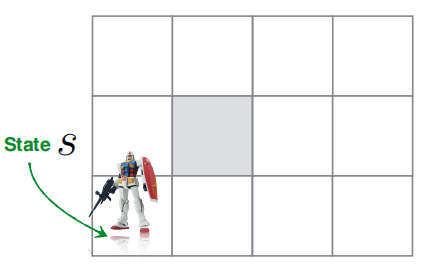
\includegraphics[width = 0.3\textwidth]{2.png}}
    \subfigure[Action]{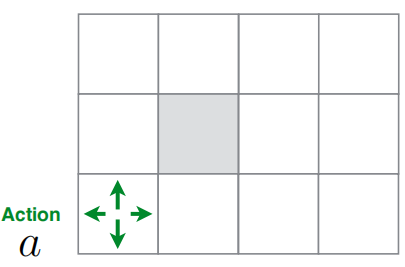
\includegraphics[width = 0.3\textwidth]{3.png}}
    \subfigure[Trajectory]{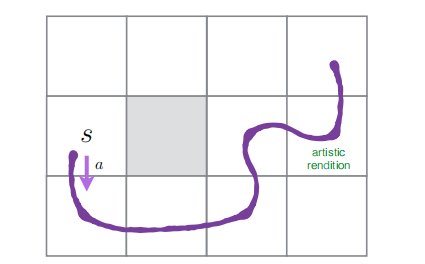
\includegraphics[width = 0.3\textwidth]{4.png}}
    
    \caption{The initial state, actions, and one trajectory of a simple example: Grid world.}
    \label{fig:1}
\end{figure}

From it, the probability of a state-action trajectory is defined as:
$$p\left(s_{0}, a_{0}, \cdots, s_{T}, a_{T}\right)$$
While the reward value is a scalar value for one trajectory is defined as:
$$r\left(s_{0}, a_{0}, \cdots, s_{T}, a_{T}\right)$$

Before moving forward to the setup of the Markov Decision Process, some concept definitions are needed.
\begin{align*}
    \centering
    & s \in S \quad \textrm{State} \\
    & a \in A_s \quad \textrm{Action} \\
    & p(s^{'} |s, a) \quad \textrm{State Transition Dynamic} \\
    & r(s^{'} |s, a) \quad \textrm{Reward function} \\
    & p_0(s) \quad \textrm{State prior} \\
    & \pi (a|s) \quad \textrm{Policy} \\
    & \gamma \quad \textrm{Discount factor}
\end{align*}
\begin{itemize}
    \item \textbf{State.} The state defines the current situation of the agent (for eg: it can be the exact position of the Robot in the house, or the alignment of its two legs, or its current posture; it depends on how you address the problem) at some time step. There can be finite or infinite states based on the situation. The example mentioned above is a discrete one, while if we define the state as the amount of oil in a vehicle, it would be continuous.
    
    \item \textbf{Action.} The choice that the agent makes at the current time step with the environment (for eg: it can move its right or left leg, or raise its arm, or lift an object, turn right or left, etc.). We know the set of actions (decisions) that the agent can perform in advance. In this example, it can be move $\{up, down, left, right\}$. Generally, it can allow us to change the current state or the environment.
    
    \item \textbf{State-Transition Dynamics.} In the real environment, there exists some uncertainty. So we are not for sure what the outcome of it even if we know the state $s$ and the action $a$. And $p(s^{'} |s, a)$ is probability to describe that, which is a the transition dynamics of the environment, and describes the probability that action $a$ in state $s$ will lead to $s^{'}$,

    \item \textbf{Reward Function.} $r(s^{'} |s, a)$ is the immediate reward received from the environment, which help us model the intention of the agents that they want to achieve. By maximizing its reward, we can get closer to what the agent want. For example, we own the amount money of $x$ and we want to earn the number of money $y$. Therefore, the reward function can be the inversely proportional to the difference from the target money.
    
    \item \textbf{State prior.} $p_0(s)$ is the initial state probability, which describes the probability of the environment or the agent being initialized to state $s_0$.
    
    \item \textbf{Policy.} As a probability distribution, a policy is the thought process behind picking an action. In practice, it is a probability distribution assigned to the set of actions. Highly rewarding actions will have a high probability and vice versa. If the agent follow the policy $\pi$, it will perform the $s$ with the probability $\pi (a|s)$ under the condition that the current state is $a$.
    
    \item \textbf{Discount factor.} The variable $\gamma \in$ [0, 1] is the discount factor. The intuition behind using a discount is that there is no certainty about the future rewards; i.e., as important it is to consider the future rewards to increase the Return, it is also equally important to limit the contribution of the future rewards to the Return (Since you can’t be 100\% sure of the future). When we look at an agents behavior over a series of time steps, we generally like to sum all of the rewards at every time step to get the return of the trajectory. In this sum, we can choose to multiply future rewards by a power of $\gamma$ to control the value of weights that we put in the future rewards.
\end{itemize}

\subsection{Factorization and Procedure of MDP}

As a sequential decision making algorithm, we can factorize the MDP to a temporal sequence of variables. As defined above, a trajectory as a sequence of states and actions $\zeta = \{s_0, a_0, s_1, a_1, ..., s_T, a_T\}$. The joint distribution of generating a trajectory $p(s_0, a_0, s_1, a_1, ..., s_T, a_T)$ and a reward function $r(s_0, a_0, s_1, a_1, ..., s_T, a_T)$, which is a scalar value for one trajectory. In this way, the state $s_t$ can capture all the relevant information and we can factorize the MDP after knowing the transition dynamics $p(s_{t+1}|s_t, a_t)$, a policy $\pi(a_t|s_t)$, and the Markov property. The equation is as below:
\begin{align*}
p(s_0, a_0, ..., s_T, a_T) = p_0(s_0)\,\Pi_{t=0}^{T-1}\,p(s_{t+1}|s_t, a_t)\pi(a_t|s_t)
\end{align*}
We will only acquire one feedback based on the whole sequence. And there are many possible factorizations of the return which can be defined as follows:
\begin{align*}
    r(s_0, a_0, s_1, a_1, ..., s_T, a_T) =  & r(s_0, a_0, s_1) + r(s_1, a_1, s_2) + ...  & \textrm{or}\\
      & r(s_0, a_0) + r(s_1, a_1) + ... & \textrm{or}\\
      & r(s_0) + r(s_1) + ...
\end{align*}

Figure~\ref{fig:process} mainly shows the whole procedure of the MDP. From the figure, we can clearly observe that every state except the initial one are determined by the previous state and action.
\begin{figure}[H]
\centering
    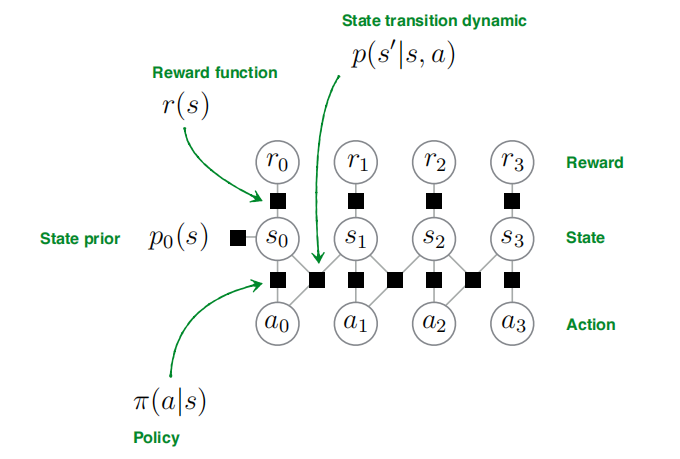
\includegraphics[width=0.7\textwidth]{process.png}
    \caption{The whole procedure of the MDP.}
	\label{fig:process}
\end{figure}

From the sub-figure 4 of Figure~\ref{fig:procedure}, we can know that though we have the previous state and conducted action, there is still a small chance to get thing wrong. The reason is that there exists some external factor such as noise and so on. In that way, it may be wrong under certain condition.
\begin{figure}[H]
    \centering
    \subfigure[Action]{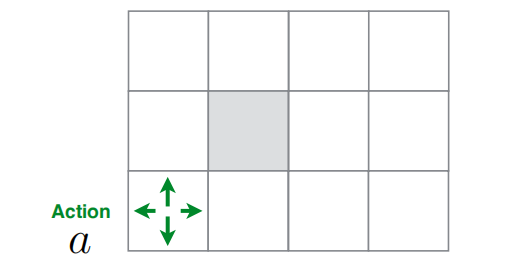
\includegraphics[width = 0.45\textwidth]{2-1.png}}
    \subfigure[Policy]{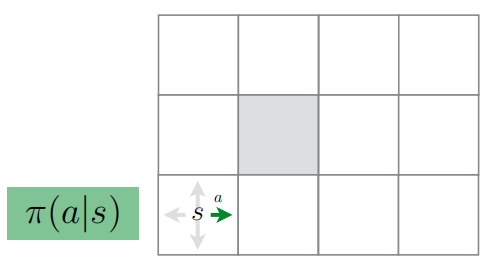
\includegraphics[width = 0.45\textwidth]{2-2.png}}
    
    \subfigure[State transition dynamic]{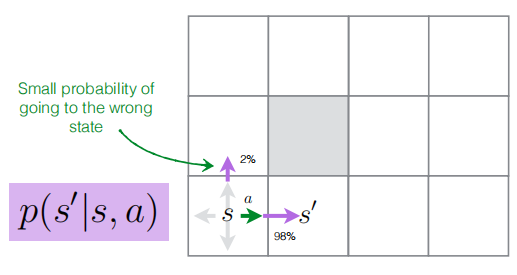
\includegraphics[width = 0.45\textwidth]{2-3.png}}
    \subfigure[Reward]{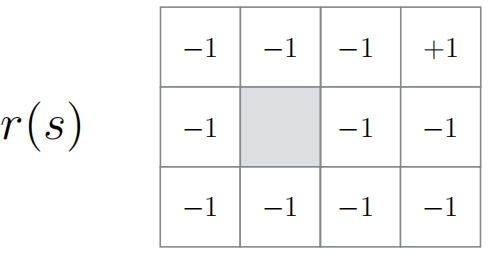
\includegraphics[width = 0.45\textwidth]{2-4.png}}
    
    \caption{The state, policy, state transition dynamic, and reward of the Grid world.}
    \label{fig:procedure}
\end{figure}


\subsection{Mathematic of the MDP}

\subsubsection{Value Function}

As the model of reinforcement learning needs to model the future, we should also know how to evaluate the performance of the modeling, which is what the value function does.
%
For a trajectory, the value function gives a feedback. And there are two major forms of value function: state value function $V^{\pi}(s)$ which gives a feedback of a trajectory starting in state $s$, and a action value function $Q^{\pi}(s, a)$ which gives a feedback of a trajectory starting in state $s$ and performing action $a$.

\textbf{State Value Function}
The state value function can be written out as:
$$V^{\pi}(s)=\mathbb{E}_{p}\left[r_{0}+r_{1}+r_{2}+\cdots \mid s_{0}=s\right], $$

in this equation, $\pi$ is the followed policy; $s$ is the starting state; $p$ is the distribution with the value of:
$$p(s_0, a_0, s_1, a_1, \cdots) = p_0(s_0) p(s1|s_0,a_0) p(a_0|s_0) p(s_2|s_1,a_1) p(a_1|s_1)\cdots$$
%
The value function can be defined with respect to different time horizons. The Infinite horizon return is defined as follows:
$$ V^{\pi}(s)=\mathbb{E}_{p}\left[r_{0}+r_{1}+r_{2}+\cdots \mid s_{0}=s\right],$$
while the finite horizon return is defined as follows:
$$ V^{\pi}(s)=\mathbb{E}_{p}\left[r_{0}+r_{1}+r_{2}+\cdots r_{T} \mid s_{0}=s\right],$$
and the infinite horizon discounted return is defined as follows:
$$ V^{\pi}(s)=\mathbb{E}_{p}\left[\gamma^{0} r_{0}+\gamma^{1} r_{1}+\gamma^{2} r_{2}+\cdots \mid s_{0}=s\right].$$
The infinite horizon discounted return is reasonable since we need to focus more on the recent state and care less about the future ones. In that way, we should model them by multiplying a discount parameter.



\textbf{State-Action Value Function}

The state-action value function means that the total feedback of a trajectory starting in the state $s$ and corresponding action $a$:

$$Q^{\pi}(s, a)=\mathbb{E}_{p}\left[\gamma^{0} r\left(s_{0}\right)+\gamma^{1} r\left(s_{1}\right)+\gamma^{2} r\left(s_{2}\right)+\cdots \mid s_{0}=s, a_{0}=a\right].$$

From the equations of $V^{\pi}(s)$ and $Q^{\pi}(s, a)$, we can find the connection between them below:

$$V^{\pi}(s)=\sum_{a} \pi(a \mid s) Q^{\pi}(s, a)$$

The process have been listed below: 

\begin{align*}
V^{\pi}(s) &=\mathbb{E}\left[\sum_{t=0}^{\infty} \gamma^{t} r_{t} \mid s_{0}=s\right] \text{A refined version of the $V^{\pi}(s)$ equation.} \\
&=\sum_{s_{1: \infty}, a_{0: \infty}} p\left(s_{1: \infty}, a_{0: \infty}\right)\left[\sum_{t=0}^{\infty} \gamma^{t} r_{t} \mid s_{0}=s\right] \text{It is a mean of all the possible state in the trajectory,} \\ & \text{so for every state and corresponding action, we should multiply the probability of it with reward } \\ & \text{function.Finally sum them together.}\\
&=\sum_{s_{1: \infty}, a_{0}: \infty} \pi\left(a_{0} \mid s_{0}=s\right) p\left(s_{1: \infty}, a_{1: \infty}\right)\left[\sum_{t=0}^{\infty} \gamma^{t} r_{t} \mid s_{0}=s\right] \text{Split the first probability since it equals } \\ & \text{to the probability from the state $s$ to take the action $a_0$.} \\
&=\sum_{a} \pi\left(a_{0}=a \mid s_{0}=s\right) \sum_{s_{1: \infty}, a_{1: \infty}} p\left(s_{1: \infty}, a_{1: \infty}\right)\left[\sum_{t=0}^{\infty} \gamma^{t} r_{t} \mid s_{0}=s, a_{0}=a\right] \text{Split the policy from the } \\ & \text{whole sum. And sum all the possible actions together.}\\
&=\sum_{a} \pi\left(a_{0}=a \mid s_{0}=s\right) \mathbb{E}\left[\sum_{t=0}^{\infty} \gamma^{t} r_{t} \mid s_{0}=s, a_{0}=a\right] \text{The latter part equals to starting from a state } \\ & \text{$s$ and an action $a$.}\\
&=\sum_{a} \pi(a \mid s) Q^{\pi}(s, a)
\end{align*}

\subsubsection{Bellman Equation}
It describe the recurrent relationship between value functions under a policy. We can find its definition in the Figure below:

\begin{figure}[H]
\centering
    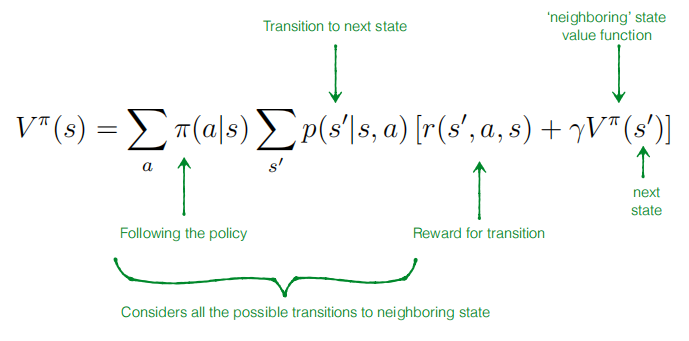
\includegraphics[width=0.7\textwidth]{BE.png}
    \caption{The Bellman Equation.}
	\label{fig:process}
\end{figure}
The process can be explained as follows. For the first sum, it sums for all the possibility of all action $a$ that for state $s$ can take. The second sum is the possibility to reach the state of $s^{'}$ under the condition of state $s$ and action $a$. The last part is the reward when transferring to $s^{'}$ and corresponding reward starting from $s^{'}$.

The process of obtaining the equations of $V^{\pi}(s_0)$ and $Q^{\pi}(s_0, a_0)$ have been listed below: 

\begin{align*}
V^{\pi}(s_0) &=\mathbb{E}\left[\gamma^{0} r_{0} + \gamma^{1} r_{1} +\gamma^{2} r_{2} + \cdots \mid s_{0}\right] \text{Original equation.} \\
&=\mathbb{E}\left[\sum_{t=0}^{\infty} \gamma^{t} r_{t} \mid s_{0}\right] \text{A refined version of the $V^{\pi}(s)$ equation.} \\
&=\mathbb{E}\left[r_{0} + \sum_{t=1}^{\infty} \gamma^{t} r_{t} \mid s_{0}\right] \text{Extract $r_0$ from the equation.} \\
&=\sum_{a_{0: \infty}}\sum_{s_{1: \infty}} p\left(s_{1: \infty}, a_{0: \infty}\right)\left[r_0 + \sum_{t=1}^{\infty} \gamma^{t} r_{t} \mid s_{0}\right] \text{In this line, we need to separately add different actions } \\ & \text{$a$ and states $s$ together. For each state, we should sum the probability that for all possible initial} \\ & \text{actions. And then, we should sum up all the probabilities that can reach different neighbour states.} \\
&= \sum_{a_0}\sum_{s_1} p(s_1\mid s_{0}, a_{0}) \pi\left(a_{0} \mid s_{0}\right) \{r_0 + \sum_{a_{1: \infty}} \sum_{s_{2: \infty}} p\left(s_{2: \infty}, a_{1: \infty}\right) \left[\sum_{t=1}^{\infty} \gamma^{t} r_{t} \mid s_{1}\right] \} \text{Keep action $a_0$ and } \\ & \text{state $s_1$ outside and move the sum to infinity inside the bracket.}\\
\end{align*}
\begin{align*}
V^{\pi}(s_0)&=\sum_{a_0}\sum_{s_1} p(s_1\mid s_{0}, a_{0}) \pi\left(a_{0} \mid s_{0}\right) \{r_0 + \mathbb{E} \left[\sum_{t=1}^{\infty} \gamma^{t} r_{t} \mid s_{1}\right] \} \text{The latter part equals to starting from a} \\ & \text{state $s_1$.}\\
&=\sum_{a_0} \pi\left(a_{0} \mid s_{0}\right) \sum_{s_1} p(s_1\mid s_{0}, a_{0}) \{r_0 + \gamma V^{\pi}(s_1)\}
\end{align*}

\begin{align*}
Q^{\pi}(s_0, a_0) &=\mathbb{E}\left[\gamma^{0} r_{0} + \gamma^{1} r_{1} +\gamma^{2} r_{2} + \cdots \mid s_{0}, a_{0}\right] \text{Original equation.} \\
&=\mathbb{E}\left[\sum_{t=0}^{\infty} \gamma^{t} r_{t} \mid s_{0}, a_{0} \right] \text{A refined version of the $V^{\pi}(s_{0}, a_{0})$ equation.} \\
&=\mathbb{E}\left[r_{0} + \sum_{t=1}^{\infty} \gamma^{t} r_{t} \mid s_{0}, a_{0}\right] \text{Extract $r_0$ from the equation.} \\
&=\sum_{s_{1: \infty}} p\left(s_{1: \infty}, a_{0: \infty}\right)\left[r_0 + \sum_{t=1}^{\infty} \gamma^{t} r_{t} \mid s_{0}, a_{0}\right] \text{Since the initial action has been ensured, we only } \\ & \text{sum all the possible probabilities that reach its neighbours.} \\
&=\sum_{s_{1}} p\left(s_{1}\mid s_{0}, a_{0}\right)\{r_0 + \mathbb{E}\left[\sum_{t=1}^{\infty} \gamma^{t} r_{t} \mid s_{1}\right]\} \text{This time, we transfer the state $s_0$ to its neighbour } \\ & \text{$s_1$ by leveraging action $a_0$. Therefore, the inside equation become the mean of starting from } \\ & \text{state $s_1$.} \\
&=\sum_{s_{1}} p\left(s_{1}\mid s_{0}, a_{0}\right)\{r_0 + \sum_{a_{1}}\pi(a_{1}\mid s_{1})\mathbb{E}\left[\sum_{t=1}^{\infty} \gamma^{t} r_{t} \mid s_{1}, a_{1}\right]\} \text{We take the second action as $a_{1}$ for } \\ & \text{every neighbour and then sum the probabilities of different policies of taking different actions } \\ & \text{together.} \\
&=\sum_{s_{1}} p\left(s_{1}\mid s_{0}, a_{0}\right)\{r_0 + \sum_{a_{1}}\pi(a_{1}\mid s_{1})Q^{\pi}(s_0, a_0)\} \text{Final equation.} \\
\end{align*}



The Bellman Equations define a (recursive) relationship between value functions and are also used to derive the Bellman optimality equations. Besides, it gives us a useful constraint for optimization.

\subsubsection{Bellman Optimality Equations}

Recurrent relationship between value functions under an optimal policy. For all the appeared policy, we need to select the policy with the more reward.
%
Therefore, we can acquire the optimal equations based on $V^{\pi}(s)$ and $Q^{\pi}(s, a)$ are defined as follows: 

$$V^{\pi^{*}}(s) = \max_{a} \sum_{s^{'}} p(s^{'}\mid s,a) \left[r_t + \gamma V^{\pi^{*}}(s_{'})\right]$$

$$Q^{\pi^{*}}(s, a) = \sum_{s_{'}} p\left(s_{'}\mid s,a\right) \left[r(s) + \gamma \max_{a^{'}} Q^{\pi^{*}}(s^{'}, a^{'})\right]$$

The process of obtaining the equation of $V^{\pi^{*}}(s)$ has been listed below: 
\begin{align*}
V^{\pi^{*}}(s) &=\sum_{a} \pi(a\mid s) Q^{\pi^{*}}(s, a) \text{Sum the probability of all possible actions for $Q^{\pi^{*}}(s, a)$ with the initial } \\ & \text{action as $a$.} \\
&=\max_{a} Q^{\pi^{*}}(s, a) \text{Change the policy into a deterministic one. For the best policy, we need to select } \\ & \text{the initial action $a$ which can maximize the reward.} \\
&=\max_{a} \mathbb{E}\left[\sum_{t=0}^{\infty} \gamma^{t} r_{t} \mid s_{0}=s, a_{0}=a \right] \text{Change the $Q$ into a sum version.} \\
&=\max_{a} \mathbb{E}\left[r_0 + \sum_{t=1}^{\infty} \gamma^{t} r_{t} \mid s_{0}=s, a_{0}=a \right] \text{Divide the first reward from the equation.} \\
&=\max_{a} \sum_{s^{'}}p(s_1=s^{'} \mid s,a)\left[r_0 + \mathbb{E}\{\sum_{t=1}^{\infty} \gamma^{t} r_{t} \mid s_{1}=s^{'}\}\right] \text{Move one step from state $s$ to state $s^{'}$. } \\ & \text{Therefore, the equation inside the bracket should start from the state $s_{'}$} \\
&= \max_{a} \sum_{s^{'}} p(s^{'}\mid s,a) \left[r_t + \gamma V^{\pi^{*}}(s_{'})\right]
\end{align*}

%\section*{References}
%Include your references here. Please cite any resources you found useful.	
%Populate the refs.bib file or list your references manually. Be consistent in formatting!
{
\bibliography{refs}
\bibliographystyle{abbrv}
}

\newpage
\section{Appendix}
%This section provides any relevant background material that was not covered in the lectures, but was found to be useful for understanding the material. 
%For example, derivations, theory underlying techniques employed, etc. 

%Additionally, this section can summarizes applications or extensions of these techniques found in the literature. 
\subsection{Hierarchical Reinforcement Learning}

In the Appendix, we would like to talk about the development and some approaches about the Hierarchical Reinforcement Learning. Most research in RL is based on the theoretical discrete-time state and action formalism of the MDP. Unfortunately, it suffers from the curse of dimensionality, where the explicit state and action space enumeration grow exponentially with the number of state variables and the number of agents, respectively. So, RL has introduced Monte Carlo methods, stochastic approximation, trajectory sampling, temporal difference backups, and function approximation. However, even these methods have reached their limits. As a result, we discuss briefly in this section broad categorizations of factored, and hierarchical approaches which break up a large problem into smaller components and solving the parts.

\subsubsection{Factored Approaches}

When the state space of the MDP can be specified as a cross-product of sets of state variables
$Ei (E = E0 × E1 × ··· × En)$, it is called a factored MDP (FMDP). The concepts of state abstraction and aggregation are strongly related to the idea of a factored state space. A factored formulation also allows for system dynamics to be specified using a more natural and intuitive representation instead of an $S×S$ probability matrix per action. Representations that can describe such structure are 2-slice Dynamic Bayesian Networks DBNs [T. Dean and K. Kanazawa; “A model for reasoning about persistence and causation”] and probabilistic STRIPS operators, the former being more popular in the literature.

In [C. Boutilier, R. Dearden, and M. Goldszmidt; “Exploiting structure in policy construction”], the authors exploit such a factored state space directly, and reveal reduction in the computation and memory required to compute the optimal solution. The assumption is that the MDP is specified by a set of DBNs, one for each action, although the claim made is that it is amenable to a probabilistic STRIPS specification too. In addition to using the network structure to elicit variable independence, they use decision-tree representations of the conditional probability distributions (CPDs) to further exploit propositional independence. Next, they construct the structured policy iteration (SPI) algorithm which aggregates states for two distinct reasons: either if the states are assigned the same action by the current strategy, or if states have the same current estimated value. With the aggregation in place, the learning algorithm based on modified policy iteration only computes at the coarser level of these state partitions instead of that of the individual states. The algorithm itself is split into two phases, structured successive approximation and structured policy improvement, mirroring the two phases of classical policy iteration. It is important to note that SPI will see fewer advantages if the optimal strategy cannot be compactly represented by a tree structure, and for the reason that there is still big overhead in finding the state partitions.

In [R. A. Howard; Dynamic Programming and Markov Processes], Algebraic Decision Diagrams (ADDs) replace the decision-tree learning of SPI for the value function and strategy representation. The paper deals with a very large MDP (about 63 million states) and shows that the learned ADD value function representation is considerably more compact than the corresponding learned decision tree in most cases. However, a big disadvantage of using ADDs is that the state variables must be boolean, which makes the modified state space larger than the original.

In order to solve large weakly coupled FMDPs, the state space of the original MDP is divided into regions that comprise sub-MDPs which run concurrently (the original MDP is a cross-product of the sub-MDPs) [N. Meuleau, M. Hauskrecht, K. Kim; “Solving very large weakly coupled Markov decision processes”]. It is assumed that states variables are only associated with a particular task and the numbers of resources that can be allocated to the individual tasks are constrained; these global constraints are what cause the weak coupling between the sub-MDPs. Their approach contains two phases: an offline phase that computes the optimal solutions (value functions) for the individual sub-MDPs and an online phase that uses these local value functions to heuristically guide the search for global resource allocation to the subtasks.

One class of methods for solving weakly coupled FMDPs involves the use of linear value function approximation. In [E. Hansen and Z. Feng; “Dynamic programming for POMDPs using a factored state representation”], the authors present two solution algorithms (based o approximate linear and dynamic programming) that approximate the value functions using a linear combination of basis functions, each basis function only depending on a small subset of the state variables. In [P. Poupart, C. Boutilier, R. Patrascu, and D. Schuurmans; “Piecewise linear value function approximation for factored MDPs”], a general framework is proposed that can select a suitable basis set and modify it based on the solution quality. Further, they use piecewise linear combination of the subtask value functions to approximate the optimal value function for the original MDP. The above approaches to solving FMDPs are classified under decision-theoretic planning in that they need a perfect model (transition and reward) of the FMDP. The work in [T. Degris, O. Sigaud, and P.-H. Wuillemin; “Learning the structure of factored markov decision processes in reinforcement learning problems”] proposes the SDYNA framework that can learn in large FMDPs without initial knowledge of their structure. SDYNA incrementally builds structured representations using incremental decision-tree induction algorithms that learn from the observations made by the agent.


\end{document} % Done!


